\documentclass[a4paper]{article}
\usepackage[utf8]{inputenc}
\usepackage[left=2.5cm,right=2.5cm,top=2.5cm,bottom=2.5cm]{geometry}
\usepackage{amsmath}
\usepackage{amsfonts}
\usepackage{amssymb}
\usepackage{graphicx}
\usepackage{fancyhdr}
\usepackage{titlesec}
\usepackage{enumitem}
\usepackage{booktabs}
\usepackage{longtable}
\usepackage{url}
\usepackage{abstract}
\usepackage{caption}
\usepackage{scrextend} % For arbitrary font sizes
\changefontsizes{13pt} % Set exactly 13pt font size

% Header configuration
\pagestyle{fancy}
\fancyhf{}
\renewcommand{\headrulewidth}{0.5pt}
\lhead{\small Molecular Biology Laboratory, Department of Biotechnology}
\rhead{\small \thepage}
\chead{}
\lfoot{}
\rfoot{}
\cfoot{}

% Section formatting
\titleformat{\section}{\normalfont\Large\bfseries}{\thesection.}{0.5em}{}
\titleformat{\subsection}{\normalfont\large\bfseries}{\thesubsection.}{0.5em}{}
\titleformat{\subsubsection}{\normalfont\normalsize\bfseries}{\thesubsubsection.}{0.5em}{}

% Customizing the title section
\makeatletter
\renewcommand{\@maketitle}{
    \noindent
    \begin{minipage}[c]{0.1\textwidth}
        
\includegraphics[width=40px]{Images/bachkhoa_logo.png}
    \end{minipage}%
    \begin{minipage}[c]{0.9\textwidth}
        \quad Ho Chi Minh City University of Technology (HCMUT), VNU-HCM
    \end{minipage}
    \par
    \vskip 0.5em
    \hrule
    \vskip 2em
    \begin{center}
    {\huge\bfseries ANIMAL CELL TECHNOLOGY: \par}
    {\huge\bfseries PRIMARY CELL ISOLATION FROM SHRIMP HEPATOPANCREAS  \par}
    \vskip 2em
    {\large Dinh Chan Phong\textsuperscript{1,2}, Tran Huu Dat\textsuperscript{1,2}, Dinh Nguyen Chinh Nghia\textsuperscript{1,2}, Hoang My Dung\textsuperscript{1,2,*} \par}
    \vskip 1.5em
    {\small \textsuperscript{1} Department of Biotechnology, Faculty of Chemical Engineering, Ho Chi Minh City University of Technology (HCMUT) \par}
    {\small \textsuperscript{2} Office for International Study Programs, Ho Chi Minh City University of Technology (HCMUT), 268 Ly Thuong Kiet Street, Dien Hong Ward, Ho Chi Minh City, Vietnam \par}
    \vskip 1em
    {\small * Corresponding author: hoangmydung@hcmut.edu.vn \par}
    \end{center}
}
\makeatother

\begin{document}
\sloppy % Allow more flexible word spacing to avoid hyphenation

\maketitle

\begin{abstract}
This study presents a standardized laboratory workflow for the isolation and establishment of a primary cell suspension from shrimp hepatopancreatic tissue (\textit{Penaeus monodon}). The procedure integrated mechanical mincing with enzymatic dissociation using 0.25\% Trypsin-EDTA in Leibovitz L-15 medium, followed by sequential filtration through 100 $\mu$m and 40 $\mu$m mesh to ensure optimal single-cell recovery. The resulting suspension was concentrated via centrifugation at 500g for 10 minutes. Cell viability and density were subsequently quantified using the Trypan blue exclusion assay in a 1:1 dilution ratio via hemocytometer analysis. The protocol successfully yielded a viable primary cell suspension, demonstrating that the synergy of mechanical and enzymatic treatments is an effective approach for harvesting crustacean cells. However, the observed viability of 18.4\% suggests that standard mammalian dissociation parameters may be suboptimal for sensitive crustacean tissues. These findings provide a foundational methodology and critical baseline data for downstream applications in marine biotechnology, pathobiology, and in vitro cellular assays.
\end{abstract}

\noindent\textbf{Keywords:} Shrimp; Primary cell culture; Hepatopancreas; Enzymatic dissociation; Trypan blue exclusion; Cell viability; L-15 Medium.

\vskip 2em
\hrule
\vskip 2em

\section{Introduction}

Animal cell technology has revolutionized the fields of medicine, pharmacology, and marine biotechnology. The ability to maintain and manipulate cells \textit{in vitro} allows for the investigation of normal cellular physiology, the testing of toxicological effects of new compounds, and the production of high-value biologicals such as viral vaccines, monoclonal antibodies, and recombinant glycoproteins \cite{3}. Central to these applications is the establishment of a primary cell culture—cells derived directly from animal tissue through mechanical or enzymatic dissociation.

In the context of marine biotechnology, crustacean cell culture, particularly from shrimp species like \textit{Penaeus monodon}, has gained significant attention due to the economic importance of the aquaculture industry. The shrimp hepatopancreas serves as a vital organ for metabolism, digestion, and detoxification, making it a primary target for pathobiological studies and viral infection assays (e.g., White Spot Syndrome Virus - WSSV). However, crustacean cells are notoriously difficult to culture \textit{in vitro} compared to mammalian counterparts, often exhibiting slow growth, high sensitivity to standard dissociation agents, and a finite lifespan \cite{1, 6}.

This laboratory report details the isolation of a primary cell suspension from the shrimp hepatopancreas. The workflow utilizes Leibovitz L-15 medium, a formulation specifically designed for maintaining cells in standard atmospheric conditions without the need for $CO_2$ supplementation \cite{2}. The procedure combines mechanical mincing with trypsinization to liberate individual cells, followed by viability assessment using the Trypan Blue exclusion method. The primary objective is to evaluate the efficacy of this standardized protocol in yielding a viable and concentrated cell population suitable for downstream research.

\section{Theoretical Background}
\subsection{Principles of Primary Cell Culture}
Primary culture refers to the stage of the culture after the cells are isolated from the tissue and proliferated under appropriate conditions until they occupy all of the available substrate (i.e., reach confluence). At this stage, the culture must be subcultured by transferring it to a new vessel with fresh growth medium to provide more room for continued growth.

Isolation methods generally fall into two categories:
\begin{enumerate}
    \item \textbf{Mechanical Dissociation:} The tissue is chopped or minced into small fragments.
    \item \textbf{Enzymatic Dissociation:} Proteolytic enzymes are used to digest the extracellular matrix and cell-adhesion molecules. Trypsin, a serine protease, is the most commonly used agent, often combined with EDTA (a chelating agent) to sequester divalent cations ($Ca^{2+}, Mg^{2+}$) that facilitate cell-cell adhesion \cite{3}.
\end{enumerate}

\subsection{Media and Environmental Requirements}
For successful \textit{in vitro} maintenance, the medium must provide essential nutrients, including glucose (energy source), amino acids (building blocks), salts (osmolarity maintenance), and vitamins (co-factors). For crustacean cells, the medium must also account for the unique physiological conditions of the organism, such as higher osmolarity compared to mammalian systems. Leibovitz L-15 medium is preferred in many marine studies because it uses galactose and sodium pyruvate instead of glucose to prevent the rapid accumulation of acidic metabolic byproducts, thus maintaining a stable pH in air \cite{2}.

\subsection{Cell Viability and Counting}
The Trypan Blue exclusion assay is the standard method for determining cell viability. The principle is based on membrane integrity: live cells with intact membranes exclude the dye and appear clear/refractive under a microscope, whereas dead cells with compromised membranes take up the dye and appear blue. Quantification is performed using a hemocytometer (Neubauer chamber), which allows for the calculation of cell density based on a known volume ($10^{-4}$ mL per large square) \cite{4, 5}.

\section{Materials and Methods}
\subsection{Experimental Workflow}
The experimental procedure for primary cell isolation followed a sequential process of tissue preparation, dissociation, and analysis, as illustrated in \textit{Figure \ref{fig:workflow}}.

\begin{figure}[htbp]
    \centering
    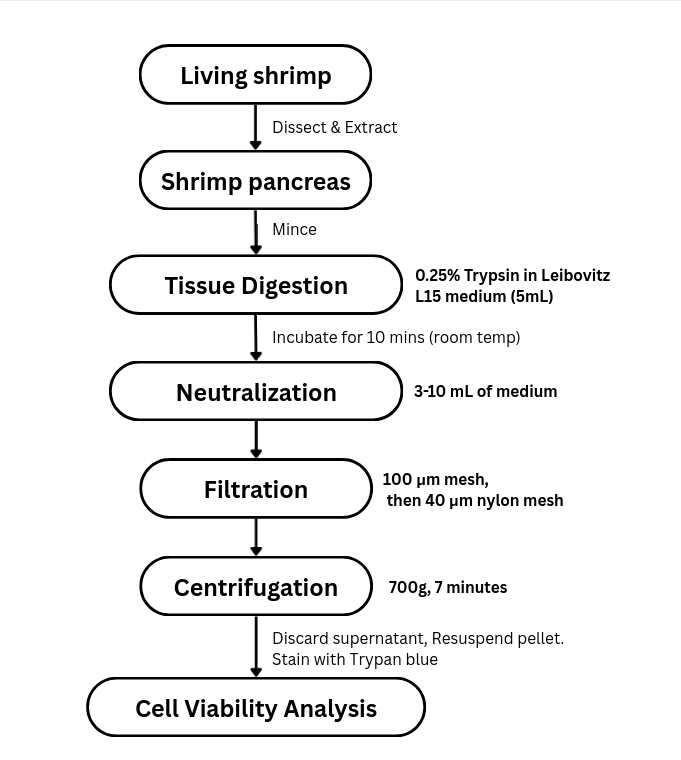
\includegraphics[width=0.8\textwidth]{Images/workflow.png}
    \caption{Detailed workflow of primary cell isolation from shrimp hepatopancreas.}
    \label{fig:workflow}
\end{figure}

\subsection{Biological Material and Aseptic Preparation}
Freshly harvested shrimp (\textit{Penaeus monodon}) were used as the tissue source. All procedures were conducted within a Class II Laminar Flow Cabinet to ensure a sterile environment. Surgical instruments were sterilized using 70\% ethanol and flame sterilization. The shrimp were surface-disinfected with 70\% ethanol before dissection.

\subsection{Reagents and Instrumentation}
Table \ref{tab:reagents} summarizes the key reagents and equipment used during the isolation and analysis phases.

\begin{table}[htbp]
\centering
\caption{Key Reagents and Equipment Specifications}
\label{tab:reagents}
\begin{tabular}{@{}lll@{}}
\toprule
Component & Specification / Concentration & Function \\
\midrule
\textbf{Basal Medium} & Leibovitz L-15 (Gibco) & Nutrient supply and pH buffering \\
\textbf{Dissociation Agent} & 0.25\% Trypsin-EDTA & Enzymatic cleavage of cell adhesions \\
\textbf{Disinfectant} & 70\% Ethanol & Aseptic surface treatment \\
\textbf{Vital Stain} & 0.4\% Trypan Blue & Viability differentiation \\
\textbf{Filtration} & 100 $\mu$m and 40 $\mu$m Nylon Mesh & Removal of tissue debris/clumps \\
\textbf{Equipment} & Hemocytometer (Neubauer) & Manual cell quantification \\
\textbf{Equipment} & Digital Microcentrifuge & Cell concentration and washing \\
\bottomrule
\end{tabular}
\end{table}

\subsection{Tissue Processing and Enzymatic Digestion}
Aseptic surgical techniques were employed to excise the hepatopancreas from the shrimp. The isolated tissue was mechanically minced into fragments ($<1$ mm$^3$) to maximize the surface area-to-volume ratio \cite{3}. Subsequently, the tissue fragments were suspended in 5 mL of Leibovitz L-15 medium supplemented with 0.25\% Trypsin-EDTA. Enzymatic dissociation was performed at 25$^\circ$C for 10 minutes with periodic gentle agitation.

\subsection{Filtration and Concentration}
Post-incubation, the enzymatic activity was neutralized by the addition of 3--10 mL of fresh L-15 medium. The resulting homogenate was passed through a sequential filtration system (100 $\mu$m followed by 40 $\mu$m) to isolate a single-cell suspension. The filtrate was collected in sterile tubes and centrifuged at 500 g for 10 minutes at room temperature.

\subsection{Resuspension and Viability Assessment}
The supernatant was aspirated, and the cell pellet was carefully resuspended in 1 mL of L-15 medium. Cell density and viability were quantified using a hemocytometer following 1:1 dilution with Trypan Blue \cite{4, 5}.


\section{Results \& Discussion}
\subsection{Primary Cell Recovery and Viability}
The isolation of primary cells from the shrimp hepatopancreas (\textit{Penaeus monodon}) was quantified using a Neubauer hemocytometer. Following a 1:1 dilution with 0.4\% Trypan Blue, the suspension was analyzed for total cell density and membrane integrity. The observed data across five major squares of the grid is presented in Table \ref{tab:viability}.

\begin{table}[htbp]
\centering
\caption{Hemocytometer Counts and Viability Analysis of Isolated Hepatopancreatic Cells}
\label{tab:viability}
\setlength{\tabcolsep}{12pt}
\renewcommand{\arraystretch}{1.2}
\begin{tabular}{lcccc}
\toprule
\textbf{Grid Square} & \textbf{Total (T)} & \textbf{Live (L)} & \textbf{Dead (D)} & \textbf{Viability (\%)} \\
\midrule
Top    & 61  & 15 & 46  & 24.6\% \\
Left   & 46  & 12 & 34  & 26.1\% \\
Center & 64  & 14 & 50  & 21.9\% \\
Right  & 64  & 6  & 58  & 9.4\% \\
Bottom & 64  & 8  & 56  & 12.5\% \\
\midrule
\textbf{Total / Average} & \textbf{299} & \textbf{55} & \textbf{244} & \textbf{18.4\%} \\
\bottomrule
\end{tabular}
\end{table}

\subsection{Quantitative Analysis}
The following calculations determine the cell concentration and total yield for the 1 mL final suspension:
\begin{enumerate}[leftmargin=*]
    \item \textbf{Percentage Viability (\%V):}
    \begin{equation}
    \%V = \left( \frac{\sum \text{Live Cells}}{\sum \text{Total Cells}} \right) \times 100 = \frac{55}{299} \times 100 \approx 18.4\%
    \end{equation}

    \item \textbf{Total Cell Concentration:}
    The dilution factor (DF) is 2. The formula for cells/mL is:
    \begin{equation}
    C_{total} = \frac{\sum T}{5} \times DF \times 10^4 = \frac{299}{5} \times 2 \times 10^4 = 1.196 \times 10^6 \text{ cells/mL}
    \end{equation}

    \item \textbf{Viable (Live) Cell Concentration:}
    \begin{equation}
    C_{live} = \frac{\sum L}{5} \times DF \times 10^4 = \frac{55}{5} \times 2 \times 10^4 = 2.2 \times 10^5 \text{ live cells/mL}
    \end{equation}

    \item \textbf{Total Viable Yield:}
    For a 1 mL suspension, the total yield is $2.2 \times 10^5$ viable cells.
\end{enumerate}

\subsection{Discussion of Low Viability and Protocol Constraints}
The achieved viability of 18.4\% is notably lower than the 80--90\% benchmark typically observed in established mammalian cell lines. Several factors intrinsic to crustacean biology and the experimental protocol likely contributed to this high mortality rate:

\subsubsection{Enzymatic Sensitivity and Trypsin Toxicity}
While 0.25\% Trypsin-EDTA is the standard for mammalian cell dissociation, it may be overly aggressive for the delicate tissue of the shrimp hepatopancreas. The hepatopancreas is a multifunctional organ involved in enzyme secretion; therefore, the addition of exogenous proteases like trypsin may cause synergistic over-digestion of the cell membranes \cite{1}. Future optimizations should investigate lower concentrations (e.g., 0.1\%) or alternative enzymes such as collagenase or dispase, which are gentler on the extracellular matrix.

\subsubsection{Mechanical Stress and Fragmentation}
The initial mechanical mincing phase is critical for increasing surface area, but excessive force or prolonged mincing can lead to immediate cell lysis. The use of fine surgical scissors and maintaining the tissue in ice-cold L-15 medium during processing is essential to mitigate this physical trauma. In this experiment, the fragment size was targeted at $<1$ mm$^3$, but the lack of precise temperature control during mincing may have exacerbated cellular decay.

\subsubsection{Osmotic Pressure and Medium Composition}
Crustacean hemolymph is generally hyperosmotic compared to mammalian serum. Although Leibovitz L-15 medium is robust for atmospheric conditions, its osmolarity may require adjustment with NaCl or specialized salts to match the physiological environment of \textit{Penaeus monodon}. An osmotic mismatch leads to cell swelling or shrinkage, both of which compromise membrane integrity and result in Trypan Blue uptake.

\subsection{Implications for Downstream Applications}
Despite the low viability, the isolation of $2.2 \times 10^5$ live cells/mL provides a sufficient starting point for primary culture establishment. However, for applications such as viral propagation (e.g., WSSV assays) or genetic transformation, a higher survival rate is mandatory. The current results suggest that the "crisis phase" observed in primary cultures is particularly acute in crustaceans, where the transition from tissue to \textit{in vitro} environment requires more specialized stabilization factors, such as the inclusion of shrimp-specific growth factors or hemolymph supplementation in the medium \cite{6}.

\section{Conclusion}
The standardized protocol successfully isolated a primary cell suspension from the shrimp hepatopancreas with a concentration of $2.2 \times 10^5$ live cells/mL. The use of Leibovitz L-15 medium provided a stable pH environment for the duration of the laboratory exercise. However, the low viability of 18.4\% underscores the technical challenges in crustacean cell technology. The findings indicate that while mechanical and enzymatic dissociation is feasible, the parameters must be finely tuned to the unique physiology of marine invertebrates. Future work will focus on optimizing trypsin exposure times and medium osmolarity to enhance cellular survival and promote long-term \textit{in vitro} maintenance.

\section*{Acknowledgements}
We express our heartfelt gratitude to Dr. Hoang My Dung for her invaluable guidance. We also thank the Ho Chi Minh City University of Technology for providing laboratory facilities.

\begin{thebibliography}{9}
\bibitem{1} Shanthi, S., et al. (2015). Establishment of a primary cell culture from the hepatopancreas of tiger shrimp, \emph{Penaeus monodon}. \emph{In Vitro Cellular \& Developmental Biology - Animal}, 51(4), 358--365.
\bibitem{2} Leibovitz, A. (1963). The growth and maintenance of tissue-cell cultures in free gas exchange with the atmosphere. \emph{American Journal of Hygiene}, 78(2), 173--180.
\bibitem{3} Freshney, R. I. (2010). \emph{Culture of Animal Cells: A Manual of Basic Technique and Specialized Applications}. John Wiley \& Sons.
\bibitem{4} Cadena-Herrera, V., et al. (2015). Validation of Three Viable-Cell Counting Methods: Manual, Semi-Automated, and Automated. \emph{Biotechnology Reports}, 7, 9--16.
\bibitem{5} Strober, W. (2015). Trypan Blue Exclusion Test of Cell Viability. \emph{Current Protocols in Immunology}, 111(1), A3.B.1--A3.B.3.
\bibitem{6} Najafabadi, M. G., et al. (2016). Primary cell culture of hepatopancreas from the white leg shrimp \emph{Litopenaeus vannamei}. \emph{Journal of Coastal Life Medicine}, 4(10), 770--774.
\end{thebibliography}

\end{document}
